%% !TEX root = manual.tex

\chapter{Introduction}
\label{sec:intro}

\section{Overview}
\label{sec:intro:overview}

The \sstmacro software package provides a simulator for large-scale parallel computer architectures. 
It permits the coarse-grained study of distributed-memory applications. 
The simulator is driven from either a trace file or skeleton application. 
The simulator architecture is modular, allowing it to easily be extended with additional network models, 
trace file formats, software services, and processor models.

Simulation can be broadly categorized as either off-line or on-line.
Off-line simulators typically first run a full parallel application on a real machine,
recording certain communication and computation events to a simulation trace.
This event trace can then be replayed post-mortem in the simulator.
Most common are MPI traces which record all MPI events, and
\sstmacro provides the DUMPI utility (\ref{sec:tutorial:dumpi}) for collecting and replaying MPI traces. 
Trace extrapolation can extend the usefulness of off-line simulation by estimating large or untraceable system scales without   
having to collect a trace, but it is limited.

We turn to on-line simulation when the hardware or applications parameters need to change.
On-line simulators instead run real application code, allowing native C/C++/Fortran to be compiled directly into the simulator.
\sstmacro intercepts certain function calls, estimating how much time passes rather than actually executing the function.
In MPI programs, for example, calls to MPI\_Send are linked to the simulator instead of passing to the real MPI library.
If desired, \sstmacro can actually be a full MPI \emph{emulator}, delivering messages between ranks and replicating the behavior of a full MPI implementation.

Although \sstmacro supports both on-line and off-line modes, on-line simulation is encouraged because
event traces are much less flexible, containing a fixed sequence of events.
Application inputs and number of nodes cannot be changed. 
Without a flexible control flow, it also cannot simulate dynamic behavior like load balancing or faults.
On-line simulation can explore a much broader problem space since they evolve directly in the simulator.

For large, system-level experiments with thousands of network endpoints, high-accuracy cycle-accurate simulation is not possible,
or at least not convenient.
Simulation requires coarse-grained approximations to be practical.
\sstmacro is therefore designed for specific cost/accuracy tradeoffs.
It should still capture complex cause/effect behavior in applications and hardware, but be efficient enough to simulate at the system-level. 
For speeding up simulator execution, we encourage \textit{skeletonization}, discussed further in Chapter \ref{chap:appsAndSkeletonization}. 
A high-quality skeleton is an application model that reproduces certain characteristics with only limited computation.  
We also encourage uncertainty quantification (UQ) for validating simulator results.
Skeletonization and UQ are the two main elements in the ``canonical'' \sstmacro workflow (Figure \ref{fig:workflow}).

\begin{figure}[t]
  \centering
    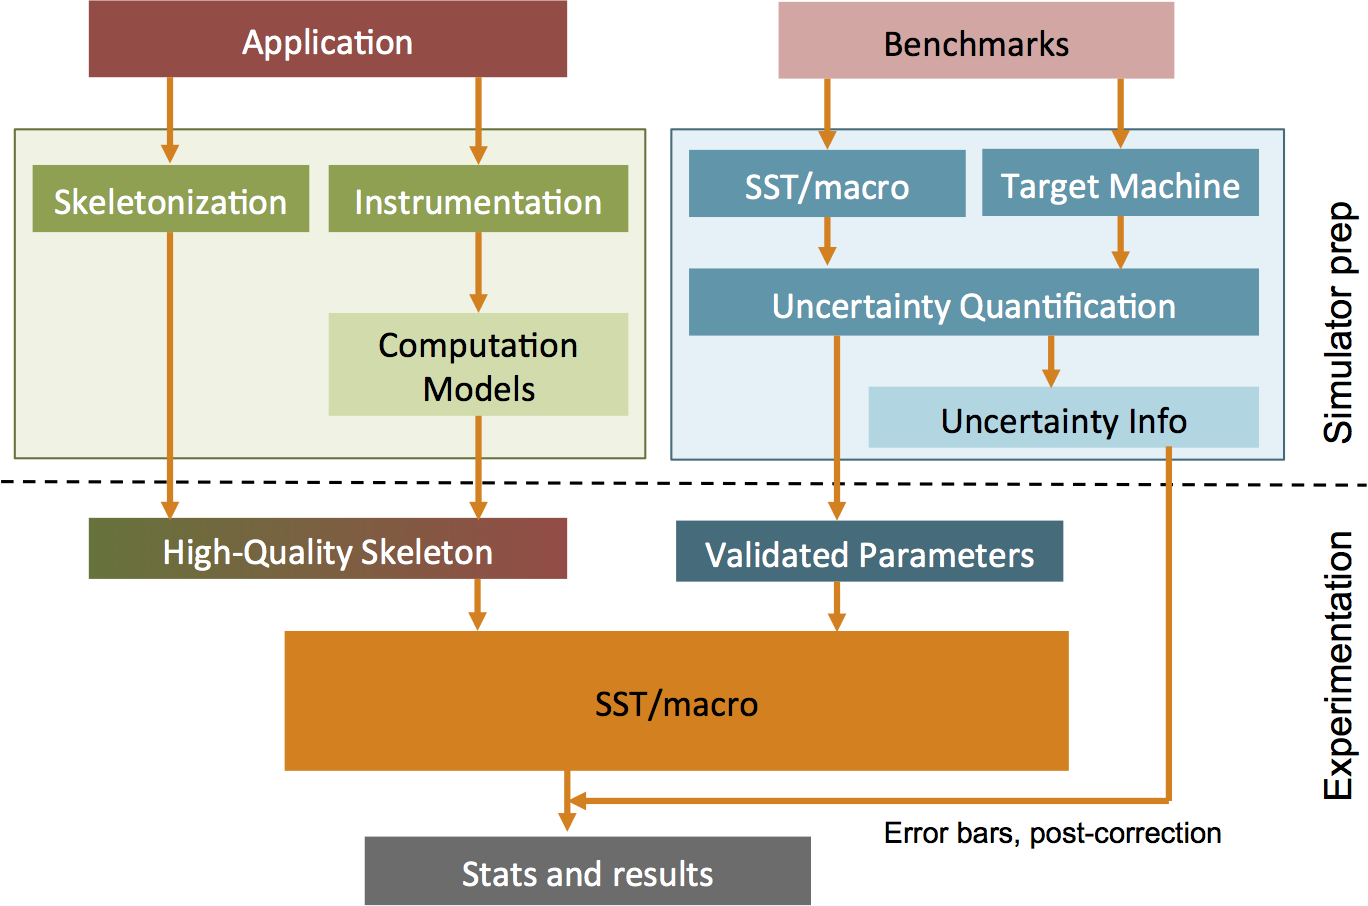
\includegraphics[width=0.99\columnwidth]{figures/workflow.png}
      \caption{SST/macro workflow.}
      \label{fig:workflow}
\end{figure}

\section{Currently Supported}
\label{sec:intro:supported}

\subsection{Programming APIs}
\label{subsec:intro:apis}

Because of its popularity, MPI is one of our main priorities in providing programming model support.  
We currently test against the MPICH test suite. All tests compile, so you should never see compilation errors.  
However, since many of the functions are not typically used in the community, we only test commonly-used functions.   
See Section \ref{subsec:issues:mpi} for functions that are not supported.  
Functions that are not implemented will throw a \inlinecode{unimplemented_error}, reporting the function name. 

\subsection{Analysis Tools and Statistics}
\label{subsec:intro:toolsandstats}
The following analysis tools are currently available in \sstmacro.
Some are thoroughly tested. Others have undergone some testing, but are still considered Beta.  Others have been implemented, but are relatively untested.

\subsubsection{Fully tested}
\label{subsubsec:intro:fulltestedtools}
\begin{itemize}
\item Call graph: Generates callgrind.out file that can be visualized in either KCacheGrind or QCacheGrind. More details are given in \ref{sec:tutorials:callgraph}.
\item Spyplot: Generates .csv data files tabulating the number of messages and number of bytes sent between MPI ranks. \sstmacro can also directly generate a PNG file. Otherwise, the .csv files can be visualized in the plotting program Scilab. More details are given in \ref{sec:tutorials:spyplot}.
\item Fixed-time quanta (FTQ): Generates a .csv data tabulating the amount of time spent doing computation/communication as the application progresses along with a Gnuplot script for visualization as a histogram. More details are given in \ref{sec:tutorials:ftq}
\end{itemize}

\section{Known Issues and Limitations}
\label{sec:intro:issues}

\subsection{MPI}
\label{subsec:issues:mpi}

Everything from MPI 2 is implemented with a few exceptions noted below.  
The following are \textit{not} implemented (categorized by MPI concepts):

\subsubsection{Communicators}
\label{subsubsec:issues:mpi:comm}

\begin{itemize}
\item Anything using or having to do with Inter-communicators (\inlinecode{MPI_Intercomm_create()})
\item Topology communicators
\end{itemize}

\subsubsection{Datatypes and Addressing}
\label{subsubsec:issues:mpi:types}

\begin{itemize}
\item Complicated use of \inlinecode{MPI_LB} and \inlinecode{MPI_UB} to define a struct, and collections of structs (MPI test 138). 
\item Changing the name of built-in datatypes with \inlinecode{MPI_Type_set_name()} (MPI test 171).
\item \inlinecode{MPI_Create_darray()}, \inlinecode{MPI_Create_subarray()}, and \inlinecode{MPI_Create_resized()}
\item \inlinecode{MPI_Pack_external()}, which is only useful for sending messages across MPI implementations apparently.
\item \inlinecode{MPI_Type_match_size()}  - extended fortran support
\item Use of \inlinecode{MPI_BOTTOM} (relative addressing).  Use normal buffers. 
\item Using Fortran types (\eg \inlinecode{MPI_COMPLEX}) from C.
\end{itemize}


\subsubsection{Info and Attributes}
\label{subsubsec:issues:mpi:info}

No \inlinecode{MPI_Info_*}, \inlinecode{MPI_*_keyval}, or \inlinecode{MPI_Attr_*} functions are supported.

\subsubsection{Point-to-Point}
\label{subsubsec:issues:mpi:ptpt}

\begin{itemize}
\item \inlinecode{MPI_Grequest_*} functions (generalized requests).
\item Use of testing non-blocking functions in a loop, such as:


\begin{CppCode}
while(!flag)
{
  MPI_Iprobe( 0, 0, MPI_COMM_WORLD, &flag, &status );
}
\end{CppCode}

For some configurations, simulation time never advances in the MPI\_Iprobe call. 
This causes an infinite loop that never returns to the discrete event manager. 
Even if configured so that time progresses, the code will work but will take a very long time to run.
	
\end{itemize}


\subsubsection{Collectives}
\label{subsubsec:issues:mpi:collectives}

\begin{itemize}
\item Non-commutative user-defined operators in \inlinecode{MPI_Reduce()} and \inlinecode{MPI_Allreduce()}.
\item \inlinecode{MPI_Alltoallw()} is not implemented
\item \inlinecode{MPI_Exscan()} is not implemented
\item \inlinecode{MPI_Reduce_Scatter_block()} is not implemented.
\item \inlinecode{MPIX_*} functions are not implemented 
\item Calling MPI functions from user-defined reduce operations (MPI test 39; including \inlinecode{MPI_Comm_rank}).
\end{itemize}


\subsection{Fortran}
\label{subsec:issues:fortran}

\sstmacro previously provided some experimental support for Fortran90 applications. 
This has been discontinued for the foreseeable future.
For profiling existing apps written with Fortran, DUMPI traces can still be generated. 

